\documentclass[11pt]{article}
\usepackage{setspace}
\setstretch{1}
\usepackage{amsmath,amssymb, amsthm}
\usepackage{graphicx}
\usepackage{bm}
\usepackage[hang, flushmargin]{footmisc}
\usepackage[colorlinks=true]{hyperref}
\usepackage[nameinlink]{cleveref}
\usepackage{footnotebackref}
\usepackage{url}
\usepackage{listings}
\usepackage[most]{tcolorbox}
\usepackage{inconsolata}
\usepackage[papersize={8.5in,11in}, margin=1in]{geometry}
\usepackage{float}
\usepackage{caption}
\usepackage{esint}
\usepackage{url}
\usepackage{enumitem}
\usepackage{subfig}
\usepackage{wasysym}
\newcommand{\ilc}{\texttt}
\usepackage{etoolbox}
\usepackage{algorithm}
\usepackage{changepage}
% \usepackage{algorithmic}
\usepackage[noend]{algpseudocode}
\usepackage{tikz}
\usetikzlibrary{matrix,positioning,arrows.meta,arrows}
\patchcmd{\thebibliography}{\section*{\refname}}{}{}{}
% \PassOptionsToPackage{hyphens}{url}\usepackage{hyperref}

\providecommand{\myceil}[1]{\left \lceil #1 \right \rceil }
\providecommand{\myfloor}[1]{\left \lfloor #1 \right \rfloor }


\begin{document}



\title{\textbf{CSDS 455: Homework 8}}

\author{Shaochen (Henry) ZHONG, \ilc{sxz517}}
\date{Due and submitted on 09/21/2020 \\ Fall 2020, Dr. Connamacher}
\maketitle

\section*{Problem 1}
\textbf{W.T.S $\lambda(G) \leq \delta(G)$:} Let $v \in V(G)$ with $\delta(v) = \delta(G)$, this suggest by removing every edges connected to $v$ we can clearly have disconncted part (the isolated $v$). This suggest $\lambda(G) = \delta(G)$.

However it is possible to have $\delta(V) < \delta(G)$, in the below example we have $\delta(G) = 2$, however by simply remove the $AB$ edge we can have a disconncted graph. Thus, $\lambda(G) \leq \delta(G)$.

\begin{figure}[H]
    \centering
    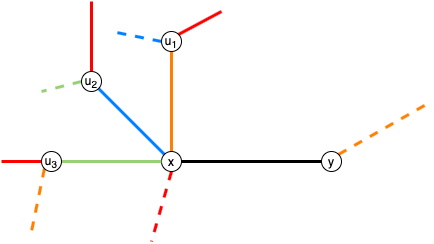
\includegraphics[width=0.45\linewidth]{{fig/fig_p1_1.png}}
    \label{fig:1_1}
\end{figure}

\textbf{W.T.S $\kappa(G) \leq \lambda(G)$:}

We know that we may have $\kappa(G) = \lambda(G)$ in a sense of $P2$ (two-vertex line), where to break it into a disconncted graph we will have $\kappa(G) = \lambda(G)$. However, it is possible to have $\kappa(G) < \lambda(G)$. In the below example we will need to remove edge $AC$ and $CB$ to make $G$ disconncted, which suggest $\lambda(G) = 2$; but we can also make $G$ disconncted by removing $C$, which yields a $\kappa(G) = 1$. Thus, we have $\kappa(G) \leq \lambda(G)$.\newline

\begin{figure}[H]
    \centering
    
\includegraphics[width=0.45\linewidth]{{fig/fig_p1_2.png}}
    \label{fig:1_2}
\end{figure}

Combine with the above to findings, we have $\kappa(G) \leq \lambda(G) \leq \delta(G)$.

\section*{Problem 2}

With a 1-dimentional cube, which is a line, the connectivity is trivially 1. With a 2-dimentional cube, which is a square, the connectivity is 2 (removing two non-adjacient vertices). For the base of induction, we assume a $d$-dimentional cube has a connectivity of $d$.

Since we can build a $d+1$-dimentional cube with two $d$-dimentional cubes, and do a perfect matching between them. This suggest $d+1$-dimentional cube has a connectivity of $d+1$. As one $d$-dimentional cube, needs to remove a minimum of $d$ vertices to disconnect internally, and it will need to remove a matching vertex from the other $d$-dimentional cube to make this $d+1$-dimentional cube become disconnected.\newline

As we have $d$ and $d + 1$ to be hold for the induction, we may conclude that a $d+1$-dimentional cube has a connectivity of $d+1$, as $\kappa(G) = d$.


\section*{Problem 3}

\begin{figure}[H]
    \centering
    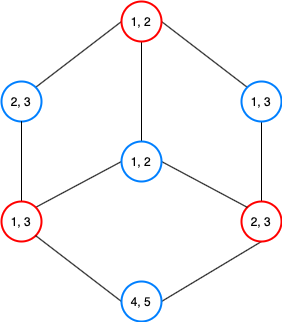
\includegraphics[width=0.45\linewidth]{{fig/fig_p3.png}}
    \label{fig:3}
\end{figure}

With $\lambda(G) = 1$ we know the cut-edge must be a bridge. So at the two sides of the bridge (we denote them as $H_1$ and $H_2$) we should also have two 3-regular subgraphs. Known that the smallest (in terms of number of vertuces) 3-regular graph will have $4$ vertices, call this $K_3_{min}$, however we can't get a bridge with two of $K_3_{min}$ graph without breaking the 3-regular property. So we will insepct the next smallest $K_3$, which has $5$ vertices, and we can build a bridge upton two of them as shown above.
\section*{Problem 4}








% \section{References}
%
% \nocite{*}
% \raggedright
% \bibliography{references.bib}
% \bibliographystyle{plain}


\end{document}